\chapter{Organisasi atau Lingkungan Kerja Praktik}
Dalam pelaksanaan kerja praktik, mahasiswa menjadi bagian dari tim proyek PT Akhdani Reka Solusi. Bab ini menjelaskan gambaran organisasi perusahaan, hubungan pengelolaan personel dengan pelaksanaan proyek, posisi mahasiswa, serta lingkup dan jadwal pekerjaannya.

\section{Profil dan Struktur Organisasi Perusahaan}\label{sec:struktur-perusahaan}
PT Akhdani Reka Solusi bergerak dalam penyediaan layanan teknologi informasi. Bidang layanannya mencakup pengembangan dan pemeliharaan perangkat lunak, integrasi sistem dan intelijen bisnis, penyediaan tenaga teknologi informasi, serta solusi pengelolaan properti. Lingkup tersebut mempertemukan pekerjaan rekayasa perangkat lunak dengan kebutuhan operasional pelanggan, baik melalui pembangunan aplikasi maupun integrasi dengan sistem yang sudah tersedia \citep{ars-onboarding}.

Pada tingkat perusahaan, Dewan Direksi terdiri atas fungsi \textit{President Director}, \textit{Director of Finance}, dan \textit{Director of Human Resources}. Bahan \textit{onboarding} memperlihatkan tiga kelompok \textit{Engineering Manager} (EM)\label{istilah:em}, yaitu EM Alpha, EM Bravo, dan EM Charlie, serta \textit{Supporting Group}. \textit{Supporting Group} mencakup fungsi administrasi keuangan dan \textit{Human Capital}. Gambar~\ref{fig:struktur-perusahaan} memperlihatkan susunan tersebut secara ringkas \citep[hlm.~7]{ars-onboarding}.

\begin{figure}[htbp]
\centering
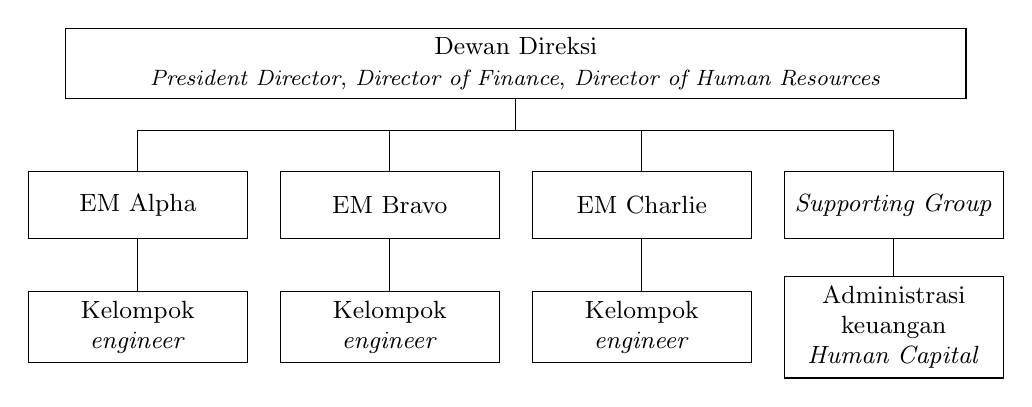
\begin{tikzpicture}[
  font=\small,
  box/.style={draw,align=center,minimum height=0.85cm,text width=2.55cm},
  line/.style={draw}]
\node[box,text width=11.2cm] (bod) at (0,0)
  {Dewan Direksi\\\footnotesize \textit{President Director}, \textit{Director of Finance}, \textit{Director of Human Resources}};
\node[box] (alpha) at (-4.8,-1.8) {EM Alpha};
\node[box] (bravo) at (-1.6,-1.8) {EM Bravo};
\node[box] (charlie) at (1.6,-1.8) {EM Charlie};
\node[box] (support) at (4.8,-1.8) {\textit{Supporting Group}};
\draw[line] (bod.south) -- (0,-0.85);
\draw[line] (-4.8,-0.85) -- (4.8,-0.85);
\foreach \name in {alpha,bravo,charlie,support}
  \draw[line] (\name.north) -- (\name.north |- 0,-0.85);
\node[box] (eng-a) at (-4.8,-3.35) {Kelompok \textit{engineer}};
\node[box] (eng-b) at (-1.6,-3.35) {Kelompok \textit{engineer}};
\node[box] (eng-c) at (1.6,-3.35) {Kelompok \textit{engineer}};
\node[box] (admin) at (4.8,-3.35) {Administrasi keuangan\\\textit{Human Capital}};
\draw[line] (alpha) -- (eng-a);
\draw[line] (bravo) -- (eng-b);
\draw[line] (charlie) -- (eng-c);
\draw[line] (support) -- (admin);
\end{tikzpicture}

\caption{Gambaran struktur perusahaan dan kelompok pengelolaan personel, disarikan dari materi \textit{onboarding}}
\label{fig:struktur-perusahaan}
\end{figure}

Pengelolaan \textit{engineer} oleh EM berlangsung lintas proyek. EM menjadi pihak yang diajak berkoordinasi mengenai ketersediaan \textit{engineer} dan kebutuhan penempatan personel. Ketika muncul persoalan kinerja \textit{engineer}, pembahasannya juga dapat melibatkan EM. Sementara itu, \textit{Project Manager} (PM)\label{istilah:pm} mengoordinasikan pelaksanaan pekerjaan pada proyek, termasuk kebutuhan personel, pembagian pekerjaan, dan perkembangan pelaksanaan. Dengan demikian, hubungan PM dengan EM merupakan koordinasi pengelolaan sumber daya manusia dan kebutuhan proyek. Perbedaan fungsi ini membantu menjelaskan bahwa seorang \textit{engineer} memiliki konteks pengelolaan personel di perusahaan sekaligus penugasan pada tim proyek.

Budaya kerja perusahaan menekankan pengerjaan yang sesuai kebutuhan, pembelajaran berkelanjutan, dan penyelesaian pekerjaan dengan komunikasi yang jelas. Prinsip tersebut didukung oleh nilai dedikasi, disiplin, akuntabilitas, sikap melayani, dan komunikasi \citep{ars-culture}. Dalam lingkungan kerja praktik, pemahaman budaya ini berkaitan dengan tanggung jawab menyampaikan perkembangan, menjelaskan kendala, serta mempelajari teknologi yang diperlukan untuk menyelesaikan penugasan.

\section{Tim Proyek dan Posisi Mahasiswa}\label{sec:tim-proyek}
Mahasiswa melaksanakan kerja praktik pada tim pengembangan sistem pengelolaan alur kerja. Struktur tim proyek memperlihatkan PM yang didukung oleh fungsi analisis bisnis, analisis sistem, koordinasi proyek, pengembangan, DevOps, penjaminan kualitas, dan dokumentasi. Fungsi-fungsi tersebut menghubungkan kebutuhan, rancangan, implementasi, serta pemeriksaan hasil pekerjaan \citep[hlm.~10]{struktur-tim}.

Gita Marshelina berperan sebagai PM dan pembimbing perusahaan. Kelompok pengembang dipimpin oleh Ervan Julianus sebagai \textit{Team Lead Dev}. Pada bagan proyek, Muhammad Usgan berada dalam kelompok \textit{Senior Dev}, sedangkan Muhammad Ra'if Alkautsar berada dalam kelompok \textit{Junior Dev}. Sebutan kelompok tersebut menjelaskan penempatan dalam tim; peran kerja praktik Ra'if adalah \textit{Software Engineer Intern}. Dalam pekerjaan teknis, Ra'if didampingi oleh Muhammad Usgan.

Frederiko Eldad Mugiyono berada pada cabang \textit{Quality Assurance} (QA)\label{istilah:qa} dengan peran \textit{Quality Assurance Intern}. Penempatan ini memperlihatkan fungsi pemeriksaan kualitas yang berkoordinasi dengan pengembangan dalam proyek yang sama. Gambar~\ref{fig:koordinasi} menunjukkan posisi kedua mahasiswa dengan arsiran. Garis putus-putus menunjukkan koordinasi personel atau pendampingan teknis, sedangkan garis penuh menunjukkan pengelompokan peran dalam perusahaan atau tim proyek.

\begin{figure}[htbp]
\centering
\begin{tikzpicture}[
  font=\small,>=Stealth,
  box/.style={draw,align=center,minimum height=1cm},
  coordination/.style={dashed,<->}]
\node[box,text width=5.4cm] (pm) at (0,0)
  {\textit{Project Manager}\\Gita Marshelina};
\node[box,text width=2.5cm] (em) at (-5.15,0) {\textit{Engineering Manager}};
\node[box,text width=2.8cm,font=\footnotesize] (functions) at (5.05,0)
  {Analisis bisnis dan sistem\\PMO / Asisten PM\\DevOps / Dokumentasi};
\draw[coordination] (em.east) -- node[above,font=\scriptsize]{SDM} (pm.west);
\draw (pm.east) -- (functions.west);
\node[box,text width=5.3cm] (lead) at (-3.35,-2.15)
  {\textit{Team Lead Dev}\\Ervan Julianus};
\node[box,text width=5.3cm,fill=shade] (qa) at (3.35,-2.15)
  {\textit{Quality Assurance}\\\NamaFrederiko\\\footnotesize Quality Assurance Intern};
\draw (pm.south) -- (0,-0.95);
\draw (lead.north) -- (lead.north |- 0,-0.95) -- (qa.north |- 0,-0.95) -- (qa.north);
\node[box,text width=3.35cm] (senior) at (-4.9,-4.4)
  {\textit{Senior Dev}\\Muhammad Usgan\\\footnotesize Pendamping teknis Ra'if};
\node[box,text width=4.5cm,fill=shade] (junior) at (-0.2,-4.4)
  {Kelompok \textit{Junior Dev}\\\NamaRaif\\\footnotesize Software Engineer Intern};
\draw (lead.south) -- (-3.35,-3.2);
\draw (senior.north) -- (senior.north |- 0,-3.2) -- (junior.north |- 0,-3.2) -- (junior.north);
\draw[dashed,->] (senior.south) -- ++(0,-0.65)
  -| node[pos=0.25,below,font=\scriptsize]{Pendampingan teknis} (junior.south);
\end{tikzpicture}

\caption{Posisi mahasiswa dalam tim proyek dan hubungan koordinasi personel; bagian bertanda arsiran menunjukkan penempatan mahasiswa}
\label{fig:koordinasi}
\end{figure}

Kelompok EM yang menaungi Ra'if belum terkonfirmasi sehingga penempatannya tidak dihubungkan dengan EM Alpha, Bravo, atau Charlie tertentu. Kedudukan Frederiko dijelaskan berdasarkan cabang QA pada struktur tim proyek; hubungan pengelolaan personelnya dengan EM tidak diasumsikan.

\section{Gambaran Proyek dan Lingkup Pekerjaan}\label{sec:unit}
Proyek yang dikerjakan oleh tim bertujuan membangun platform untuk mendefinisikan, menjalankan, dan memantau proses bisnis melalui konfigurasi. Sebuah proses memiliki tahapan, pelaksana, aturan perpindahan, serta data yang harus diisi. Platform menghubungkan definisi tersebut dengan formulir dinamis dan pelaksanaan pekerjaan sehingga proses yang memiliki kebutuhan berbeda dapat menggunakan fondasi aplikasi yang sama \citep{rancangan-awal}.

Secara umum, repositori proses bisnis menyimpan definisi dan versi proses. Mesin alur kerja menggunakan definisi tersebut untuk mengatur keadaan serta perpindahan tahap pada suatu pekerjaan. Formulir dinamis menyediakan masukan yang berkaitan dengan tahapan, sedangkan riwayat dan dasbor membantu pengguna menelusuri pelaksanaan serta memantau perkembangannya. Pengelolaan identitas, hak akses, berkas, notifikasi, dan data referensi menyediakan layanan pendukung bagi bagian-bagian tersebut. Hubungan antarmodul dan teknologi pengembangannya dijelaskan lebih lanjut pada Bab III.

Dalam lingkungan proyek, pekerjaan dibagi menjadi tugas atau tiket yang berkaitan dengan fitur sistem. Penugasan dan komunikasi pekerjaan dilakukan melalui WhatsApp atau Microsoft 365, sedangkan perkembangan pekerjaan dibahas dalam rapat mingguan. Mahasiswa bergabung dalam pengembangan yang sudah berlangsung dan mengerjakan bagian yang ditugaskan dengan menggunakan struktur kode serta komponen yang telah tersedia.

Tabel~\ref{tab:pembagian} menunjukkan pembagian tanggung jawab kedua mahasiswa. Mahasiswa pengembang menangani perubahan antarmuka dan layanan aplikasi, sedangkan mahasiswa \textit{quality assurance} (QA) ditempatkan pada fungsi penjaminan kualitas. Rincian pekerjaan QA perlu dilengkapi oleh mahasiswa yang bersangkutan agar pembagian tugas dapat menggambarkan kontribusi masing-masing.
\begin{table}[htbp]
\caption{Pembagian tugas mahasiswa kerja praktik}\label{tab:pembagian}
\begin{tabularx}{\textwidth}{@{}P{4.7cm}Y@{}}
\toprule\textbf{Mahasiswa} & \textbf{Tanggung jawab}\\\midrule
\NamaRaif{} (\NIMRaif) & Pengembangan dasbor, pengelolaan peran dan hak akses, riwayat alur kerja, pengujian komponen, serta adaptasi layanan ke Go.\\
\NamaFrederiko{} (\NIMFrederiko) & Perancangan skenario uji, otomasi pengujian antarmuka dan API (dasbor pemantauan, \textit{master data}, proses bisnis, autentikasi), pelaporan temuan, serta pengujian regresi.\\
\bottomrule
\end{tabularx}
\end{table}

Lingkup platform lebih luas daripada kontribusi individu mahasiswa. Pengembangan repositori proses bisnis, mesin alur kerja, dan formulir dinamis menjadi pekerjaan tim secara keseluruhan. Kontribusi mahasiswa dijelaskan melalui bagian yang dikerjakan serta hubungannya dengan platform, sehingga penambahan fitur peran, riwayat, atau dasbor tidak diartikan sebagai pembangunan seluruh sistem oleh mahasiswa.

\section{Deskripsi Pekerjaan}
\subsection{Pemahaman Kebutuhan dan Kode Aplikasi}
Tahap awal dilakukan dengan mengikuti penjelasan proyek, mempelajari alur kerja sistem, dan menelaah struktur kode antarmuka serta layanan aplikasi. Pada tahap ini, mahasiswa juga mempelajari teknologi yang digunakan dalam proyek (seperti Vue), pengelolaan keadaan aplikasi, dan teknologi penyimpanan data yang digunakan dalam repositori.

\subsection{Pengembangan Antarmuka dan Integrasi Data}
Pekerjaan antarmuka dimulai dari pembuatan halaman dasbor dan komponen penyajian informasi. Data simulasi digunakan untuk mengembangkan tampilan sebelum seluruh layanan tersedia. Pekerjaan dilanjutkan dengan halaman daftar, pembuatan, detail, dan penyuntingan peran, serta penyajian riwayat alur kerja. Integrasi dilakukan dengan menyesuaikan permintaan dan respons API\label{istilah:api} yang digunakan pada setiap halaman.

\subsection{Pengembangan Layanan dan Akses Data}
Pada layanan aplikasi, pekerjaan mencakup penanganan permintaan pengelolaan peran, penyediaan data pengguna, pengaturan hak akses, dan pengambilan riwayat proses. Pengembangan juga melibatkan penyesuaian data awal, penamaan atribut, dan pesan kesalahan agar perilaku antarmuka sesuai dengan hasil pemrosesan layanan.

\subsection{Pengujian dan Perbaikan}
Mahasiswa pengembang menyusun pengujian komponen untuk halaman pengelolaan peran dan riwayat alur kerja. Perbaikan dilakukan terhadap masalah tampilan, navigasi, data yang belum diperbarui, serta penanganan kegagalan layanan.

Mahasiswa penjaminan kualitas melaksanakan pengujian independen melalui pendekatan kotak abu-abu yang memadukan pengujian antarmuka ujung ke ujung berbasis Cypress dan pengujian langsung ke antarmuka pemrograman aplikasi (API). Tahapan pengujian diawali dengan analisis spesifikasi alur kerja, perancangan skenario uji positif dan negatif, pemetaan kode sumber untuk mengidentifikasi rute layanan dan selektor pengujian, hingga implementasi skrip otomasi pengujian. Setiap anomali teknis, seperti celah otorisasi pada \textit{endpoint} peran, ketidakkonsistenan penamaan atribut selektor pengujian, serta keterbatasan interaksi menu navigasi, dicatat dan dikomunikasikan secara berkala kepada mahasiswa pengembang dan tim proyek. Hasil perbaikan yang diimplementasikan oleh pengembang kemudian diuji kembali secara regresi untuk memastikan stabilitas fungsionalitas sistem.

\subsection{Adaptasi Teknologi dan Perancangan Lanjutan}
Pergantian teknologi pada bulan Agustus diikuti oleh pembelajaran Go, penyiapan lingkungan layanan baru, dan pemindahan fitur pengelolaan peran. Pada akhir periode, pekerjaan juga mencakup penyiapan Docker untuk pengembangan lokal dan pembuatan rancangan layar pengelolaan dasbor serta \textit{widget} menggunakan Visily.

\section{Jadwal Kerja}\label{sec:jadwal}
Pelaksanaan kerja praktik berlangsung pada \PeriodeKP. Mahasiswa bekerja secara \textit{work from office} (WFO) pada Senin hingga Kamis dan \textit{work from home} (WFH) pada Jumat. Rapat mingguan dijadwalkan setiap hari Selasa pukul 09.30. Tabel~\ref{tab:tahapan} merangkum tahapan pekerjaan pengembangan selama periode tersebut.
\begin{table}[htbp]
\caption{Jadwal kegiatan pengembangan selama kerja praktik}\label{tab:tahapan}
\small
\begin{tabularx}{\textwidth}{@{}P{3.1cm}Y@{}}
\toprule\textbf{Periode} & \textbf{Kegiatan}\\\midrule
22 Juni--3 Juli & Orientasi, pembelajaran teknologi, pengembangan dasbor dan data simulasi, serta pendalaman autentikasi dan alur kerja.\\
6--17 Juli & Implementasi pengelolaan peran, integrasi layanan, penyiapan data awal, dan penyeragaman kode.\\
20--31 Juli & Pengembangan riwayat alur kerja, perbaikan navigasi dan panduan pengguna, serta pengujian komponen.\\
3--14 Agustus & Pembelajaran Go dan kerangka kerja web, penyiapan proyek, serta analisis pemindahan fitur.\\
18--28 Agustus & Adaptasi pengelolaan peran, penyesuaian autentikasi, penyiapan lingkungan lokal, dan rancangan layar.\\
31 Agustus & Penutupan periode kerja praktik dengan pemaparan dari \textit{President Director}.\\
\bottomrule
\end{tabularx}
\end{table}

Di luar pekerjaan teknis, kedua mahasiswa mengikuti kegiatan internal perusahaan dalam rangka peringatan kemerdekaan pada tanggal 18 Agustus. Catatan harian pekerjaan Muhammad Ra'if Alkautsar disajikan pada Lampiran~\ref{app:logbook}, sedangkan catatan harian dan artefak pengujian Frederiko Eldad Mugiyono disajikan pada Lampiran~\ref{app:frederiko}.

Tabel~\ref{tab:tahapan-qa} merangkum tahapan kegiatan penjaminan kualitas selama periode kerja praktik.
\begin{table}[htbp]
\caption{Jadwal kegiatan penjaminan kualitas selama kerja praktik}\label{tab:tahapan-qa}
\small
\begin{tabularx}{\textwidth}{@{}P{3.1cm}Y@{}}
\toprule\textbf{Periode} & \textbf{Kegiatan}\\\midrule
22 Juni--3 Juli & Orientasi lingkungan kerja, analisis alur proses bisnis, penyusunan skenario awal, dan implementasi otomasi pengujian dasbor operasional.\\
6--17 Juli & Perumusan konvensi selektor pengujian (\textit{data-cy}), perancangan kasus uji negatif, serta implementasi otomasi antarmuka dan API \textit{master} peran.\\
20--31 Juli & Otomasi pengujian \textit{master} entitas, konfigurasi sistem, data referensi, autentikasi, \textit{master} pengguna, dan modul proses bisnis.\\
3--14 Agustus & Penyesuaian skenario terhadap pembaruan alur proses rilis pertama, analisis purwarupa antarmuka di Visily, dan perincian kasus uji negatif alur kerja.\\
18--28 Agustus & Pengujian kasus batas validasi masukan formulir, penyesuaian skrip otomasi terhadap lingkungan penerapan baru, dan penyusunan panduan kerangka uji.\\
31 Agustus & Presentasi laporan akhir kerja praktik di hadapan pembimbing perusahaan dan tim proyek.\\
\bottomrule
\end{tabularx}
\end{table}
